% !TeX encoding = UTF-8
% !TeX program = xelatex
% !TeX spellcheck = en_US

\documentclass[degree=bachelor]{ustcthesis}
% degree    = doctor|master|bachelor
% language  = chinese|english

% 加载宏包、全部的配置
% !TeX root = ./main.tex

\ustcsetup{
  title              = {中国科学技术大学\\学位论文模板示例文档},
  title*             = {An example of thesis template for University of Science
                        and Technology of China},
  author             = {李泽平},
  author*            = {Li Zeping},
  speciality         = {数学与应用数学},
  speciality*        = {Mathematics and Applied Mathematics},
  supervisor         = {XXX~教授, XXX~教授},
  supervisor*        = {Prof. XXX, Prof. XXX},
  % date               = {2017-05-01},  % 默认为今日
  % professional-type  = {专业学位类型},
  % professional-type* = {Professional degree type},
  % secret-level       = {秘密},     % 绝密|机密|秘密,注释本行则不保密
  % secret-level*      = {Secret},  % Top secret|Highly secret|Secret
  % secret-year        = {10},      % 保密年限
}


% 加载宏包
\usepackage{graphicx}
\usepackage{booktabs}
\usepackage{longtable}
\usepackage[ruled,linesnumbered]{algorithm2e}
\usepackage{siunitx}
\usepackage{amsthm}


% 数学命令
% !TeX root = ./main.tex

% Adapted for use with ustcthesis.
% Original code is at https://github.com/goodfeli/dlbook_notation/blob/master/math_commands.tex

%%%%% NEW MATH DEFINITIONS %%%%%

\newcommand\ceil[1]{\lceil #1 \rceil}
\newcommand\floor[1]{\lfloor #1 \rfloor}


% Vectors
\newcommand\Vector[1]{\symbf{#1}}

\newcommand\0{{\Vector{0}}}
\newcommand\vzero{{\Vector{0}}}
\newcommand\1{{\Vector{1}}}
\newcommand\vone{{\Vector{1}}}

\newcommand\va{{\Vector{a}}}
\newcommand\vb{{\Vector{b}}}
\newcommand\vc{{\Vector{c}}}
\newcommand\vd{{\Vector{d}}}
\newcommand\ve{{\Vector{e}}}
\newcommand\vf{{\Vector{f}}}
\newcommand\vg{{\Vector{g}}}
\newcommand\vh{{\Vector{h}}}
\newcommand\vi{{\Vector{i}}}
\newcommand\vj{{\Vector{j}}}
\newcommand\vk{{\Vector{k}}}
\newcommand\vl{{\Vector{l}}}
\newcommand\vm{{\Vector{m}}}
\newcommand\vn{{\Vector{n}}}
\newcommand\vo{{\Vector{o}}}
\newcommand\vp{{\Vector{p}}}
\newcommand\vq{{\Vector{q}}}
\newcommand\vr{{\Vector{r}}}
\newcommand\vs{{\Vector{s}}}
\newcommand\vt{{\Vector{t}}}
\newcommand\vu{{\Vector{u}}}
\newcommand\vv{{\Vector{v}}}
\newcommand\vw{{\Vector{w}}}
\newcommand\vx{{\Vector{x}}}
\newcommand\vy{{\Vector{y}}}
\newcommand\vz{{\Vector{z}}}

\newcommand\valpha{{\Vector{\alpha}}}
\newcommand\vbeta{{\Vector{\beta}}}
\newcommand\vgamma{{\Vector{\gamma}}}
\newcommand\vdelta{{\Vector{\delta}}}
\newcommand\vepsilon{{\Vector{\epsilon}}}
\newcommand\vtheta{{\Vector{\theta}}}
\newcommand\viota{{\Vector{\iota}}}
\newcommand\vkappa{{\Vector{\kappa}}}
\newcommand\vlambda{{\Vector{\lambda}}}
\newcommand\vmu{{\Vector{\mu}}}
\newcommand\vnu{{\Vector{\nu}}}
\newcommand\vxi{{\Vector{\xi}}}
\newcommand\vpi{{\Vector{\pi}}}
\newcommand\vrho{{\Vector{\rho}}}
\newcommand\vsigma{{\Vector{\sigma}}}
\newcommand\vtau{{\Vector{\tau}}}
\newcommand\vupsilon{{\Vector{\upsilon}}}
\newcommand\vphi{{\Vector{\phi}}}
\newcommand\vchi{{\Vector{\chi}}}
\newcommand\vpsi{{\Vector{\psi}}}
\newcommand\vomega{{\Vector{\omega}}}


% Matrix
\newcommand\MATRIX[1]{\symbf{#1}}

\newcommand\mA{{\MATRIX{A}}}
\newcommand\mB{{\MATRIX{B}}}
\newcommand\mC{{\MATRIX{C}}}
\newcommand\mD{{\MATRIX{D}}}
\newcommand\mE{{\MATRIX{E}}}
\newcommand\mF{{\MATRIX{F}}}
\newcommand\mG{{\MATRIX{G}}}
\newcommand\mH{{\MATRIX{H}}}
\newcommand\mI{{\MATRIX{I}}}
\newcommand\mJ{{\MATRIX{J}}}
\newcommand\mK{{\MATRIX{K}}}
\newcommand\mL{{\MATRIX{L}}}
\newcommand\mM{{\MATRIX{M}}}
\newcommand\mN{{\MATRIX{N}}}
\newcommand\mO{{\MATRIX{O}}}
\newcommand\mP{{\MATRIX{P}}}
\newcommand\mQ{{\MATRIX{Q}}}
\newcommand\mR{{\MATRIX{R}}}
\newcommand\mS{{\MATRIX{S}}}
\newcommand\mT{{\MATRIX{T}}}
\newcommand\mU{{\MATRIX{U}}}
\newcommand\mV{{\MATRIX{V}}}
\newcommand\mW{{\MATRIX{W}}}
\newcommand\mX{{\MATRIX{X}}}
\newcommand\mY{{\MATRIX{Y}}}
\newcommand\mZ{{\MATRIX{Z}}}

\newcommand\mGamma{{\MATRIX{\Gamma}}}
\newcommand\mDelta{{\MATRIX{\Delta}}}
\newcommand\mTheta{{\MATRIX{\Theta}}}
\newcommand\mLambda{{\MATRIX{\Lambda}}}
\newcommand\mXi{{\MATRIX{\Xi}}}
\newcommand\mPi{{\MATRIX{\Pi}}}
\newcommand\mSigma{{\MATRIX{\Sigma}}}
\newcommand\mUpsilon{{\MATRIX{\Upsilon}}}
\newcommand\mPhi{{\MATRIX{\Phi}}}
\newcommand\mPsi{{\MATRIX{\Psi}}}
\newcommand\mOmega{{\MATRIX{\Omega}}}


% Tensor
\newcommand\tens[1]{\symbfsf{#1}}
\newcommand\tA{{\tens{A}}}
\newcommand\tB{{\tens{B}}}
\newcommand\tC{{\tens{C}}}
\newcommand\tD{{\tens{D}}}
\newcommand\tE{{\tens{E}}}
\newcommand\tF{{\tens{F}}}
\newcommand\tG{{\tens{G}}}
\newcommand\tH{{\tens{H}}}
\newcommand\tI{{\tens{I}}}
\newcommand\tJ{{\tens{J}}}
\newcommand\tK{{\tens{K}}}
\newcommand\tL{{\tens{L}}}
\newcommand\tM{{\tens{M}}}
\newcommand\tN{{\tens{N}}}
\newcommand\tO{{\tens{O}}}
\newcommand\tP{{\tens{P}}}
\newcommand\tQ{{\tens{Q}}}
\newcommand\tR{{\tens{R}}}
\newcommand\tS{{\tens{S}}}
\newcommand\tT{{\tens{T}}}
\newcommand\tU{{\tens{U}}}
\newcommand\tV{{\tens{V}}}
\newcommand\tW{{\tens{W}}}
\newcommand\tX{{\tens{X}}}
\newcommand\tY{{\tens{Y}}}
\newcommand\tZ{{\tens{Z}}}


% Graph
\newcommand\gA{{\mathcal{A}}}
\newcommand\gB{{\mathcal{B}}}
\newcommand\gC{{\mathcal{C}}}
\newcommand\gD{{\mathcal{D}}}
\newcommand\gE{{\mathcal{E}}}
\newcommand\gF{{\mathcal{F}}}
\newcommand\gG{{\mathcal{G}}}
\newcommand\gH{{\mathcal{H}}}
\newcommand\gI{{\mathcal{I}}}
\newcommand\gJ{{\mathcal{J}}}
\newcommand\gK{{\mathcal{K}}}
\newcommand\gL{{\mathcal{L}}}
\newcommand\gM{{\mathcal{M}}}
\newcommand\gN{{\mathcal{N}}}
\newcommand\gO{{\mathcal{O}}}
\newcommand\gP{{\mathcal{P}}}
\newcommand\gQ{{\mathcal{Q}}}
\newcommand\gR{{\mathcal{R}}}
\newcommand\gS{{\mathcal{S}}}
\newcommand\gT{{\mathcal{T}}}
\newcommand\gU{{\mathcal{U}}}
\newcommand\gV{{\mathcal{V}}}
\newcommand\gW{{\mathcal{W}}}
\newcommand\gX{{\mathcal{X}}}
\newcommand\gY{{\mathcal{Y}}}
\newcommand\gZ{{\mathcal{Z}}}


% Sets
\newcommand\sA{{\mathbb{A}}}
\newcommand\sB{{\mathbb{B}}}
\newcommand\sC{{\mathbb{C}}}
\newcommand\sD{{\mathbb{D}}}
% Don't use a set called E, because this would be the same as our symbol
% for expectation.
\newcommand\sF{{\mathbb{F}}}
\newcommand\sG{{\mathbb{G}}}
\newcommand\sH{{\mathbb{H}}}
\newcommand\sI{{\mathbb{I}}}
\newcommand\sJ{{\mathbb{J}}}
\newcommand\sK{{\mathbb{K}}}
\newcommand\sL{{\mathbb{L}}}
\newcommand\sM{{\mathbb{M}}}
\newcommand\sN{{\mathbb{N}}}
\newcommand\sO{{\mathbb{O}}}
\newcommand\sP{{\mathbb{P}}}
\newcommand\sQ{{\mathbb{Q}}}
\newcommand\sR{{\mathbb{R}}}
\newcommand\sS{{\mathbb{S}}}
\newcommand\sT{{\mathbb{T}}}
\newcommand\sU{{\mathbb{U}}}
\newcommand\sV{{\mathbb{V}}}
\newcommand\sW{{\mathbb{W}}}
\newcommand\sX{{\mathbb{X}}}
\newcommand\sY{{\mathbb{Y}}}
\newcommand\sZ{{\mathbb{Z}}}


% Random variables
\newcommand\RandomVariable[1]{\symit{#1}}

\newcommand\rA{{\RandomVariable{A}}}
\newcommand\rB{{\RandomVariable{B}}}
\newcommand\rC{{\RandomVariable{C}}}
\newcommand\rD{{\RandomVariable{D}}}
\newcommand\rE{{\RandomVariable{E}}}
\newcommand\rF{{\RandomVariable{F}}}
\newcommand\rG{{\RandomVariable{G}}}
\newcommand\rH{{\RandomVariable{H}}}
\newcommand\rI{{\RandomVariable{I}}}
\newcommand\rJ{{\RandomVariable{J}}}
\newcommand\rK{{\RandomVariable{K}}}
\newcommand\rL{{\RandomVariable{L}}}
\newcommand\rM{{\RandomVariable{M}}}
\newcommand\rN{{\RandomVariable{N}}}
\newcommand\rO{{\RandomVariable{O}}}
\newcommand\rP{{\RandomVariable{P}}}
\newcommand\rQ{{\RandomVariable{Q}}}
\newcommand\rR{{\RandomVariable{R}}}
\newcommand\rS{{\RandomVariable{S}}}
\newcommand\rT{{\RandomVariable{T}}}
\newcommand\rU{{\RandomVariable{U}}}
\newcommand\rV{{\RandomVariable{V}}}
\newcommand\rW{{\RandomVariable{W}}}
\newcommand\rX{{\RandomVariable{X}}}
\newcommand\rY{{\RandomVariable{Y}}}
\newcommand\rZ{{\RandomVariable{Z}}}

% Random vectors
\newcommand\RandomVector[1]{\symbf{#1}}

\newcommand\rvA{{\RandomVector{A}}}
\newcommand\rvB{{\RandomVector{B}}}
\newcommand\rvC{{\RandomVector{C}}}
\newcommand\rvD{{\RandomVector{D}}}
\newcommand\rvE{{\RandomVector{E}}}
\newcommand\rvF{{\RandomVector{F}}}
\newcommand\rvG{{\RandomVector{G}}}
\newcommand\rvH{{\RandomVector{H}}}
\newcommand\rvI{{\RandomVector{I}}}
\newcommand\rvJ{{\RandomVector{J}}}
\newcommand\rvK{{\RandomVector{K}}}
\newcommand\rvL{{\RandomVector{L}}}
\newcommand\rvM{{\RandomVector{M}}}
\newcommand\rvN{{\RandomVector{N}}}
\newcommand\rvO{{\RandomVector{O}}}
\newcommand\rvP{{\RandomVector{P}}}
\newcommand\rvQ{{\RandomVector{Q}}}
\newcommand\rvR{{\RandomVector{R}}}
\newcommand\rvS{{\RandomVector{S}}}
\newcommand\rvT{{\RandomVector{T}}}
\newcommand\rvU{{\RandomVector{U}}}
\newcommand\rvV{{\RandomVector{V}}}
\newcommand\rvW{{\RandomVector{W}}}
\newcommand\rvX{{\RandomVector{X}}}
\newcommand\rvY{{\RandomVector{Y}}}
\newcommand\rvZ{{\RandomVector{Z}}}

\newcommand\laplace{\mathrm{Laplace}} % Laplace distribution

\newcommand\E{\mathbb{E}}
\newcommand\Ls{\mathcal{L}}
\newcommand\R{\mathbb{R}}
\newcommand\emp{\tilde{p}}
\newcommand\lr{\alpha}
\newcommand\reg{\lambda}
\newcommand\rect{\mathrm{rectifier}}
\newcommand\softmax{\mathrm{softmax}}
\newcommand\sigmoid{\sigma}
\newcommand\softplus{\zeta}
\newcommand\KL{D_{\mathrm{KL}}}
\newcommand\Var{\mathrm{Var}}
\newcommand\standarderror{\mathrm{SE}}
\newcommand\Cov{\mathrm{Cov}}
% Wolfram Mathworld says $L^2$ is for function spaces and $\ell^2$ is for vectors
% But then they seem to use $L^2$ for vectors throughout the site, and so does
% wikipedia.
\newcommand\normlzero{L^0}
\newcommand\normlone{L^1}
\newcommand\normltwo{L^2}
\newcommand\normlp{L^p}
\newcommand\normmax{L^\infty}

\DeclareMathOperator*{\argmax}{arg\,max}
\DeclareMathOperator*{\argmin}{arg\,min}

\DeclareMathOperator{\sign}{sign}
\DeclareMathOperator{\Tr}{Tr}
\let\ab\allowbreak


% 配置图片的默认目录
\graphicspath{{figures/}}

% 用于写文档的命令
\DeclareRobustCommand\cs[1]{\texttt{\char`\\#1}}
\DeclareRobustCommand\pkg{\textsf}
\DeclareRobustCommand\file{\nolinkurl}


% hyperref 宏包在最后调用
\usepackage{hyperref}

\usepackage{subfigure}
\begin{document}

% 研究生论文:
%   封面,原创性声明和授权使用声明
%   frontmatter: 摘要,目录,[图、表清单],[符号说明]
%   mainmatter: 正文章节,参考文献
%   appendix: 附录
%   backmatter: 致谢,已发表论文列表
%
% 本科生论文:
%   封面
%   frontmatter: 致谢,目录,摘要
%   mainmatter: 正文章节,参考文献
%   appendix: 附录

\maketitle
\copyrightpage

\frontmatter
% !TeX root = ../main.tex

\begin{acknowledgements}

在研究期间,我有幸得到了两位导师的指导,他们是:我的导师清华大学交叉信息学院的张崇洁,中国科大吴锋老师。感谢给予我的悉心教导和热情帮助。

同时,感谢王同翰学长的帮助,没有他便没有这样的成果。感谢在中科大四年的学习中各位老师的教导,在他们的严谨教学中,我受益良多。感谢张旭老师在东区2103教室的管理心理学和美学课,让我在繁重的学业之外看到了一些色彩。感谢室友王立峰、常天宇、奴尔江的帮助和谈笑风生。

感谢疫情期间家人的支持,才让我能集中精力去做科研。

感谢评审论文的老师们在百忙之中抽出时间,来评审我的毕业论文。

\end{acknowledgements}
 % TODO: [chap] write acknowledgement in the end
\tableofcontents
% !TeX root = ../main.tex

\ustcsetup{
  keywords = {
    中国科学技术大学, 学位论文, \LaTeX{} 模板, 学士, 硕士, 博士
  },
  keywords* = {
    University of Science and Technology of China (USTC), Thesis,
    \LaTeX{} Template, Bachelor, Master, PhD
  },
}

\begin{abstract}
  摘要是论文内容的总结概括,应简要说明论文的研究目的、基本研究内容、 研究方法或
  过程、结果和结论,突出论文的创新之处。摘要中不宜使用公式、图表,不引用文献。
  博士论文中文摘要一般800~1000个汉字,硕士论文中文摘要一般600个汉字。英文摘要的
  篇幅参照中文摘要。

  关键词另起一行并隔写在摘要下方,一般3~8个词,中文关键词间空一字或用分号“;”隔
  开。英文摘要的关键词与中文摘要的关键词应完全一致,中间用逗号“,”或分号“;”隔开。

\end{abstract}

\begin{enabstract}
  This is a sample document of USTC thesis \LaTeX{} template for bachelor,
  master and doctor. The template is created by zepinglee and seisman, which
  orignate from the template created by ywg. The template meets the
  equirements of USTC theiss writing standards.

  This document will show the usage of basic commands provided by \LaTeX{} and
  some features provided by the template. For more information, please refer to
  the template document ustcthesis.pdf.

\end{enabstract}
 % TODO: [chap] write abstract in the end
% \listoffigures
% \listoftables
% % !TeX root = ../main.tex

\begin{notation}

  \begin{notationlist}{2em}
    \item[$\displaystyle a$] The number of angels per unit area
    \item[$\displaystyle N$] The number of angels per needle point
    \item[$\displaystyle A$] The area of the needle point
    \item[$\displaystyle \sigma$] The total mass of angels per unit area
    \item[$\displaystyle m$] The mass of one angel
    \item[$\displaystyle \sum_{i=1}^n a_i$] The sum of $a_i$
  \end{notationlist}

\end{notation}



% 也可以使用 nomencl 宏包

% \printnomenclature

% \nomenclature{$\displaystyle a$}{The number of angels per unit are}
% \nomenclature{$\displaystyle N$}{The number of angels per needle point}
% \nomenclature{$\displaystyle A$}{The area of the needle point}
% \nomenclature{$\displaystyle \sigma$}{The total mass of angels per unit area}
% \nomenclature{$\displaystyle m$}{The mass of one angel}
% \nomenclature{$\displaystyle \sum_{i=1}^n a_i$}{The sum of $a_i$}


\mainmatter


% !TeX root = ../main.tex

\chapter{绪论}
\section{研究背景}
很多现实世界的系统可以被建模成多智能体系统(MAS), 比如自动交通队伍~\cite{cao2012overview}, 智能仓库系统~\cite{nowe2012game}, 感受器网络~\cite{zhang2011coordinated}等等。而协同多智能体强化学习(MARL)提供了一个很有前景的去处理这些问题的方式,因为MARL能让智能体处理不确定的环境,以及能够逐步适应环境。近些年,协同多智能体强化学习取得了很大的进步,有很多基于深度学习的算法被提出来~\cite{foerster2018counterfactual, sunehag2018value, rashid2018qmix, son2019qtran, vinyals2019grandmaster, wang2020learning, baker2020emergent}。

\section{国内外研究现状}
为了获得可拓展性,现在的多智能体深度强化学习框架往往采用一个很简化的模式,即所有的智能体都共享以及学习一个分离的值网络或者策略网路,但是这样简单的共享往往是不够的,特别是对于一些复杂的多智能体任务。举例来说,在Adam Smith的大头针工厂里,工人必须要完成18个完全不同的子任务才能制作成一个大头针~\cite{smith1937wealth}。在这个情形下,只用一个共享的网络往往是很重的负担,因为它要同时去学很多完全不同的策略,还要去表达不同的技能。在另一方面,每个智能体都单独有一个网络也是没必要的,因为有一些工人会有相同的任务,并且各自独立也会增加计算复杂度。

所以问题就是如何能充分发挥智能体的的专业化以及动态的信息、参数共享来提高性能。

一个很自然的概念会出现,就是角色。角色是行为模式的抽象,一个角色常常专注于某些任务。拥有相似角色的智能体会有相似的行为,因而能够共享它们的经验以来提高性能。

事实上,角色理论已经在经济学、社会学和组织学中被广泛地研究了。科研人员以前也将角色概念引入到多智能体强化学习中~\cite{becht1999rope, stone1999task, depke2001roles, ferber2003agents, odell2004metamodel, bonjean2014adelfe, Lhaksmana2018role}。在这些基于角色的框架中,往往是通过任务分解、将角色与子任务联系起来来完成智能体设计的~\cite{zhu2008role}. 然而,这些工作需要利用领域知识来完成任务分解以及需要预定义每个角色的责任,这些限制了基于角色的多智能体系统应用到动态的、变化的、未知的环境中。

\section{主要工作与创新点}
为了同时利用角色理论以及深度学习方法,本项目提出了一个基于角色的多智能体强化学习框架(Role-Oriented Multi-Agent Reinforcement Learning), 并命名为ROMA.

本框架隐式地将角色概念引入到多智能体强化学习,让角色充当媒介,使得拥有相似角色的智能体能够共享它们的训练学习。为了达到这一点,本框架让拥有相似角色的智能体同时有相似的策略和子任务。

为了将角色和智能体的策略联系起来,本框架将智能体的策略决定于它自己的角色,而角色又来自又它自己的观测决定的角色空间的采样。为了将角色和子任务联系起来,本框架提出了两个损失函数,使得角色能够通过它的行为被识别出来,以及使得角色专注于某些子任务。

本文会展示,通过优化损失函数的变分估计,能得到结构良好的角色表征,以及优异的性能。

本项目的实验均是在星际争霸2微操作环境~\cite{vinyals2017starcraft, samvelyan2019starcraft}中进行的。实验结果表明,本算法通过让拥有相似角色的智能体共享策略、学习,极大地推进了多智能体强化学习的科研进程。对同质和异质环境下的角色表征的可视化也说明了学到的角色能够动态地适应环境,以及拥有相似子任务的智能体有相似的角色。除此之外,对角色演化和涌现的分析,也说明了角色驱动的子任务专业化和集体性能的提高有很大的关联。这些结果也提供了一个理解和促进智能体的某些涌现和写作的新视角。

\section{论文组织结构}
本文按如下展开,第二章讲背景知识,第三章详细地阐释了本框架,第四章分析实验结果,第五章做简要的总结和展望。
% !TeX root = ../main.tex

\chapter{基础概念与基本算法}
\section{马尔科夫决策过程}

\section{强化学习发展历程}

\section{单智能体强化学习及其算法简介}

\section{多智能体强化学习及其算法简介}

\section{星际争霸2实验环境简介}

\section{相关工作与对比}

\section{本章小结}


% !TeX root = ../main.tex

\chapter{基于角色涌现的多智能体强化学习}
本章详细描述具体的基于角色的框架,以及考虑到“角色”应该具有的诸多性质,来设计损失函数,以引导“角色”涌现的完成。本章的结构为,首先介绍角色是什么,然后角色应该具有的四种性质,再然后引入让每个智能体的效用函数都基于自己的角色的方法,进一步再根据角色的性质设计用于优化的损失函数,最后再对总的损失函数进行总结。同时,为了让本框架更加容易理解,本章在后面还附加上另一种从深度学习角度的原理阐述。

\section{角色的定义}
为了不引起混淆,简要描述一下本文使用的角色的定义。

本文的角色是对某一行为模式的抽象。它应该具有如下的表现特征:

i) \textbf{具有某一角色的智能体常常专注于某一个或某一些子任务;}

ii) \textbf{具有相似角色的智能体会有相似的行为;}

拿蚂蚁来举例,一个蚂蚁群通常分为如下的角色:工蚁、兵蚁、蚁后等,具有工蚁角色的蚂蚁通常的行为是采集食物、建造巢穴、哺育幼蚁等,如果两只蚂蚁具有相似的角色(比如都是工蚁),那么它们的行为就会相似,具体来说,在蚂蚁这个案例里,这两只蚂蚁的每日的轨迹可能是重叠的。但是反过来,不同的角色,比如工蚁和兵蚁,它们的行为轨迹就会大不相同。

最后,角色本身是复杂的概念,很难做一个完整的定义,本文只关注那些比较明显的特征。


\section{角色具有的性质}
本小节介绍本项目认为的角色应该具有的性质。

从社会学的角度来说,角色应该会拥有很复杂、广泛的性质,比如某个角色可能会在与其他角色的交互中不断演化、越来越复杂。但是完全表达这些复杂的性质是没有必要的,本项目的目的是为了利用角色这一概念中对多智能体强化学习有启发的部分,因此,考虑到有效性和可行性,角色应该要具有如下的性质:

i) \textbf{可识别性(Identifiable)}: 一个智能体的角色能够通过它的行为模式识别出来。这一性质意味着,一个角色应该是与行为模式挂钩的,这一点正符合对角色的定义,即“角色是对某一行为模式的抽象”。

ii) \textbf{专业化(Specialized)}: 具有相似角色的智能体应该专门处理相似的子任务。这一性质同时也意味着处理相似的子任务的智能体应该也是相似的角色。

iii) \textbf{动态(Dynamic)}: 一个智能体的角色应该能动态地变化,并且这种变化是为了适应环境。正如上文所说,角色会随着和环境、其他角色的交互不断演化。

iv) \textbf{通用性(Versatile)}: 涌现出来的角色应该足够不同,这样才能处理那些需要不同角色的任务。比如蚁群的生存繁衍任务,就需要工蚁、兵蚁、蚁后等角色才能完成。


\section{基于角色的智能体}
在表达上一节的性质之前,需要先设计如何让一个智能体基于角色来决策。

注意到,在现在的多智能体系统中,每个智能体$i$都有一个局部的效用函数(或者一个局部的策略函数),为了让智能体是基于自己的角色的,让该智能体的局部效用(策略)函数的参数$\theta_i$决定于它自己的角色$\rho_i$. 

同时,为了让学到的角色拥有上面表述的性质,将角色编码到随机嵌入空间(stochastic embedding space), 在这个基础上,让每个智能体$i$的角色$\rho_i$采样自一个多维高斯分布,即$\mathcal{N}(\bm{\mu}_{\rho_i}, \bm{\sigma}_{\rho_i})$.

\section{框架结构图}
为了便于后续的长文的理解,这里提前给出完整的框架图。

\begin{figure*}
    \centering
    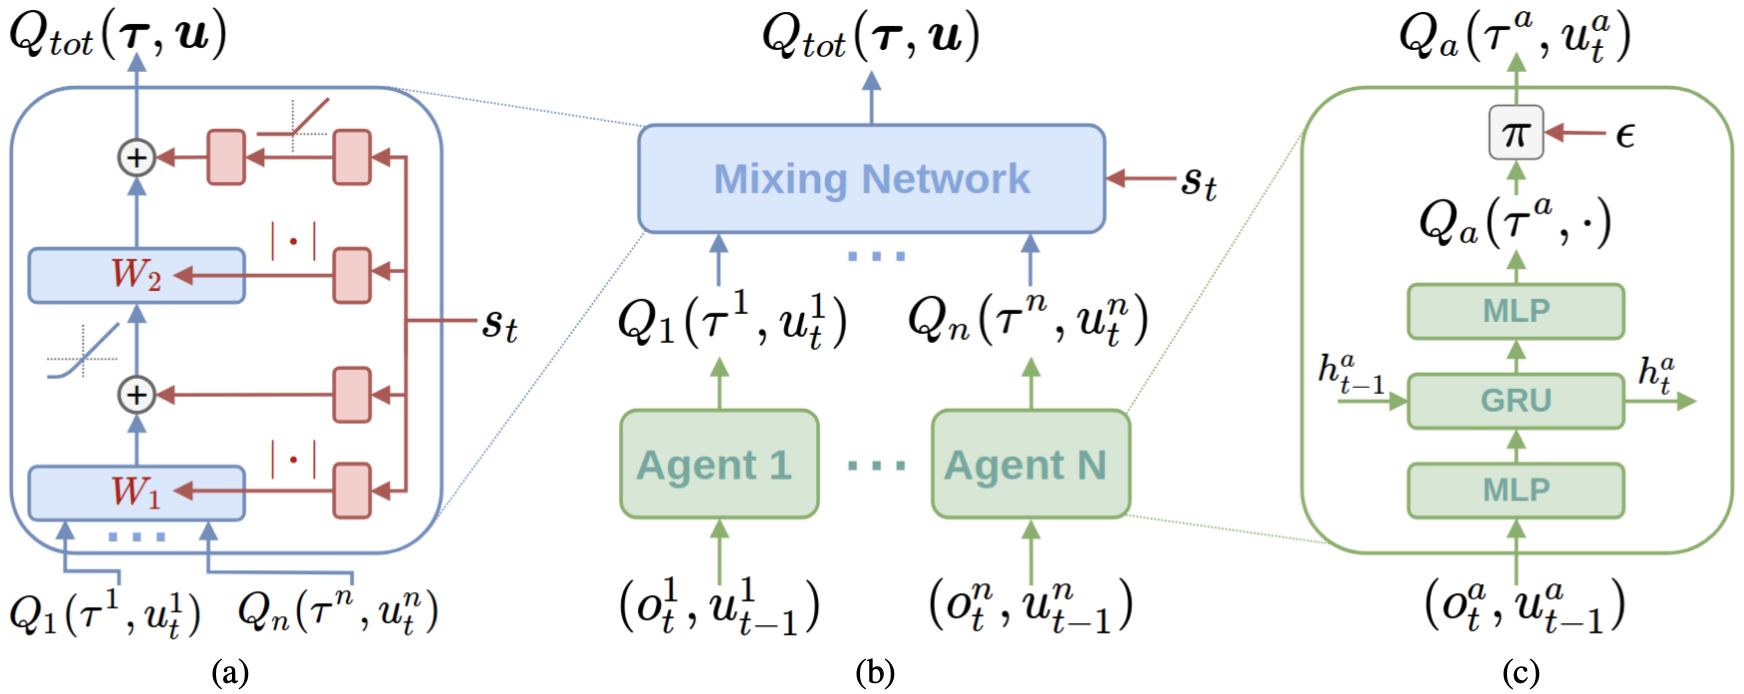
\includegraphics[width=0.8\linewidth]{figures/framework/qmix_framework.png}
    \caption{QMIX的框架图}
    \label{fig:qmix_framework}
    \note{(a)是混合网络的结构(蓝色), 它的权重和偏置是又一个超网络(hyper-net)(红色)得到的。 (b)是QMIX的整体框架结构图。(c)是局部效用函数图。}
\end{figure*}

前文叙述到,可以将智能体的局部效用函数或者局部策略函数决定于该智能体的角色,本项目在实践上使用的是局部效用函数,并且采用QMIX~\cite{rashid2018qmix}的基本框架,它的框架图为图~\ref{fig:qmix_framework}.

\begin{figure}
    \centering
    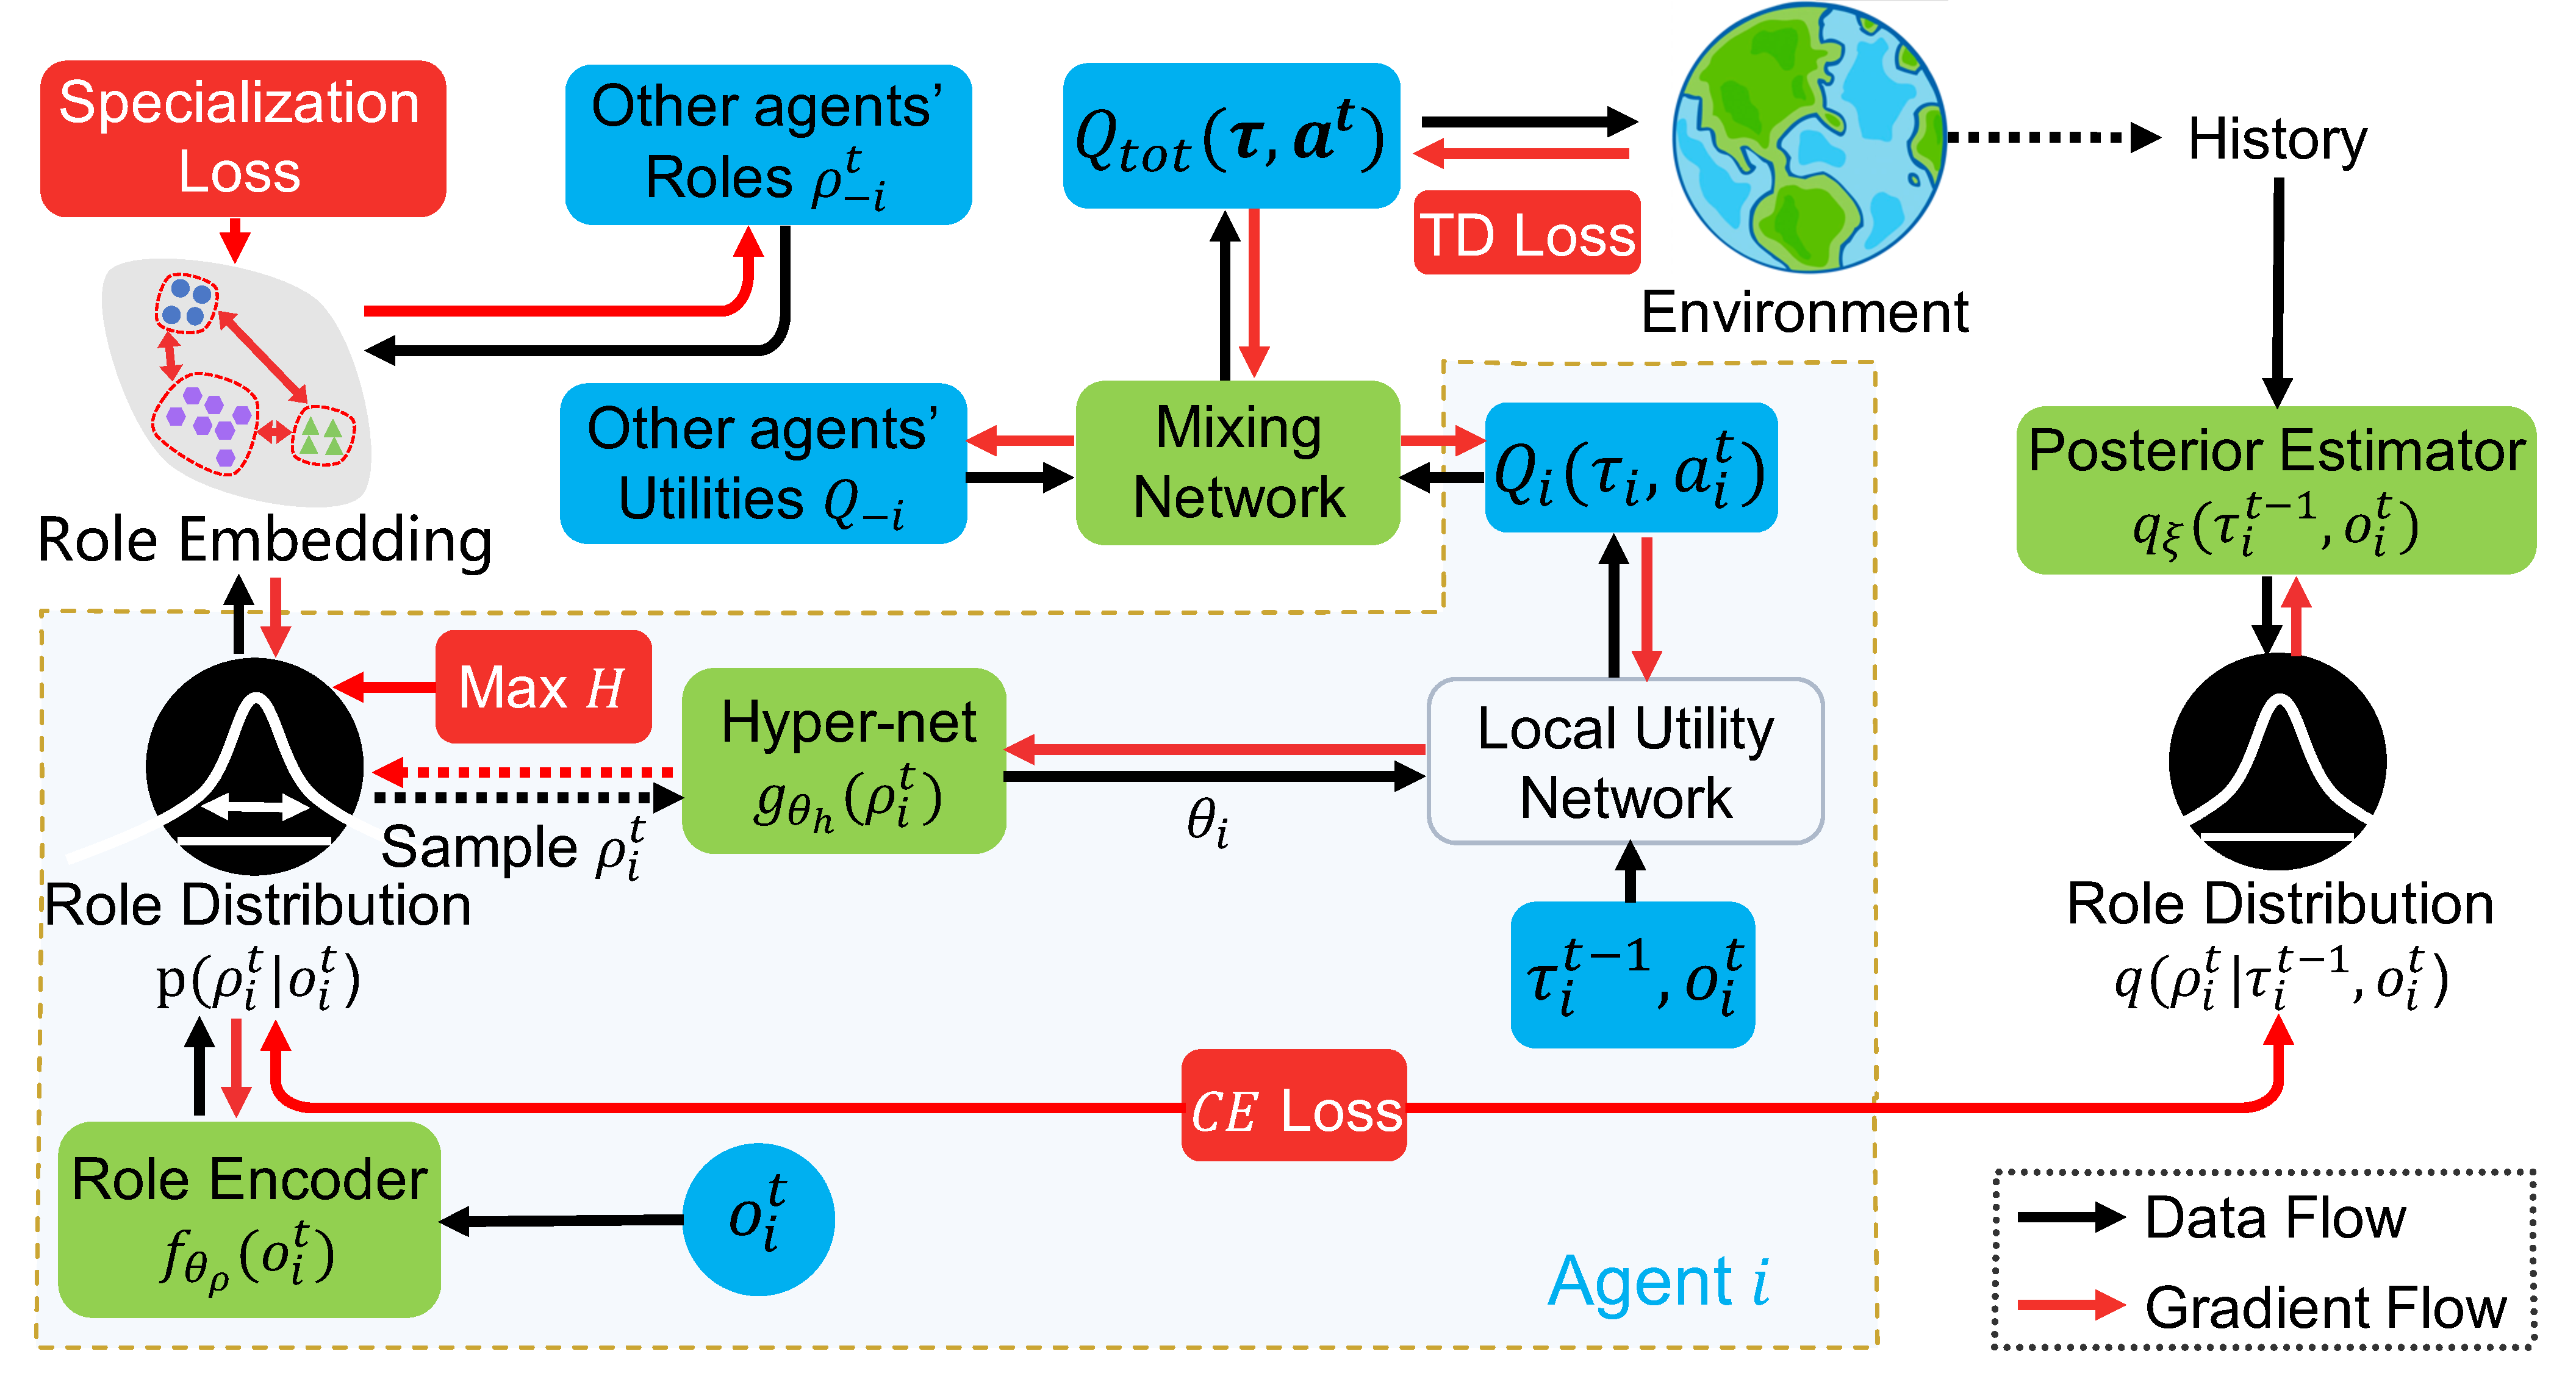
\includegraphics[width=0.95\linewidth]{figures/framework/framework.pdf}
    \caption{本项目的框架图}
    \label{fig:framework}
    \note{角色编码器产生一个在角色嵌入空间的多维高斯分布,从这个分布里采样得到一个角色,然后作为输入给一个超网络,输出得到局部效用函数的参数,即权重和偏置。局部效用函数得到的值再集中进入到一个混合网络,得到整体动作的值的一个估计。在智能体和环境以及其他智能体的交互中,个体的轨迹被收集起来,然后进入到轨迹编码器,得到角色分布的后验估计。整个框架使用端到端的方式训练。}
\end{figure}

本项目的框架图为图~\ref{fig:framework}

\section{角色的性质及损失函数设计}
前面介绍了如何将智能体基于自己的角色来决策,并且给出了基本角色应该具有的四个性质,下面将结合基本框架,设计损失函数,使得最终学到的角色满足上面的性质。

\subsection{角色的动态变化性质}
角色的动态变化性质是指,一个智能体的角色能够为了适应环而动态地变化。为了班组这个性质,将智能体的角色取决于它自己的局部观测,上文提到角色是采样自一个多维高斯分布,在此基础上,使用一个输入为智能体局部观测的可训练的神经网络$f$来学习这个多维高斯分布的参数,即$\bm{\mu}_{\rho_i}$和$\bm{\sigma}_{\rho_i}$, 完整的表达如下:
\begin{equation}
\begin{aligned}
(\bm{\mu}_{\rho_i}, \bm{\sigma}_{\rho_i}) &= f(o_i; \theta_\rho), \\
\rho_i &\sim \mathcal{N}(\bm{\mu}_{\rho_i}, \bm{\sigma}_{\rho_i}),
\end{aligned}
\end{equation}
其中,$\theta_\rho$ 是神经网络$f$的参数,$o_i$是智能体的局部观测。

得到多维高斯分布之后采样得到角色$\rho_i$, 然后该角色经过一个超网络(hyper-network)$g(\rho_i;\theta_h)$(其中$\theta_h$为该超网络的参数)处理得到局部效用函数的参数$\theta_i$. 在下文中,将会把$f$称为角色编码器(role encoder), 把$g$称为角色解码器(role decoder),这一点类似自动编码器(auto-encoder)结构。

\subsection{角色的可识别性和通用性}
注意到,上述引入角色的随机嵌入空间和将角色决定于每个智能体自己的局部观测,并不能得到一个满足通用性和可识别性的角色,因为目前没有引入别的信息来满足这一点。

\subsubsection{条件互信息建模}
% TODO: 添加熵、条件熵、交叉熵、互信息、条件互信息的背景知识
为了满足通用性,即让角色在决定于局部观测$o_i$的条件下足够地不同,可以最大化一个信息熵$H(\rho_i|o_i)$. 另一方面,为了满足可识别性,可以在给定路径$\tau_i$信息条件下最小化条件熵$H(\rho_i | \tau_i, o_i)$.

结合这两个熵,只需要去最大化$H(\rho_i | o_i) - H(\rho_i | \tau_i, o_i)$, 在数学上,这个式子等价于$I(\tau_i; \rho_i | o_i)$, 也就是关于每个智能体自己的路径$\tau_i$和基于当前观测$o_i$的角色$\rho_i$之间的的条件互信息。

\subsubsection{条件互信息的下界}
% TODO: 添加variational inference的背景知识
然而,直接去估计和最大化互信息往往是不可行的,因为它们的数值无法直接得到。为了解决这个问题,采用变分推断~\cite{wainwright2008graphical, alemi2017deep}.

引入一个变分后验估计来得到一个可以处理的关于互信息的下界,注意到这里是针对每个时刻$t$:
\begin{align*}
    I(\rho^t_i; \tau^{t-1}_i | o^t_i) & = \mathbb{E}_{\rho^t_i, \tau^{t-1}_i, o^t_i}\left[\log\frac{p(\rho^t_i | \tau^{t-1}_i, o^t_i)}{p(\rho^t_i | o^t_i)}\right] \\
    & = \mathbb{E}_{\rho^t_i, \tau^{t-1}_i, o^t_i}\left[\log\frac{q_\xi(\rho^t_i | \tau^{t-1}_i, o^t_i)}{p(\rho^t_i | o^t_i)}\right] \\ & \ \ \ \ + \mathbb{E}_{\tau^{t-1}_i, o^t_i}\left[\KL(p(\rho^t_i|\tau^{t-1}_i, o^t_i) \| q_\xi(\rho^t_i|\tau^{t-1}_i, o^t_i))\right] \\
    & \ge  \mathbb{E}_{\rho^t_i, \tau^{t-1}_i, o^t_i}\left[\log\frac{q_\xi(\rho^t_i | \tau^{t-1}_i, o^t_i)}{p(\rho^t_i | o^t_i)}\right]\stepcounter{equation}\tag{\theequation}
    \label{equ:mi}
 \end{align*}
其中,轨迹$\tau^{t-1}_i=(o_i^0, a_i^0, \cdots, o_i^{t-1}, a_i^{t-1})$, $q_\xi$是一个变分估计,它的参数是$\xi$. 另外最后一个不等式成立是因为KL散度的非负性。
% TODO: 添加KL divergence的背景知识

% TODO: 添加GRU的背景知识
分布$q_\xi$可以是任意的,这里使用一个GRU~\cite{cho2014learning}来编码每个智能体自己的历史观测和动作,这个结构称之为轨迹编码器(trajectory encoder).

为了便于最小化,公式~\ref{equ:mi}中的下界可以进一步表达成一个损失函数的形式:
\begin{align*}
    \mathcal{L}_I(\theta_\rho, \xi) = & \mathbb{E}_{(\tau^{t-1}_i, o^t_i)\sim D}\big[\mathcal{CE}[p(\rho^{t}_i | o^t_i)\| q_\xi(\rho^{t}_i | \tau^{t-1}_i, o^t_i)] - H(\rho^{t}_i | o^t_i)\big],\stepcounter{equation}\tag{\theequation}
\end{align*}
其中,$\mathcal{D}$是缓存,$H(\cdot)$是熵,$\mathcal{CE[\cdot\|\cdot]}$是交叉熵。推导如下。

\subsubsection{损失函数的推导}
上面得到关于条件互信息的如下下界:
\begin{equation}
    I(\rho^t_i; \tau^{t-1}_i | o^t_i) \ge  \mathbb{E}_{\rho^t_i, \tau^{t-1}_i, o^t_i}\left[\log\frac{q_\xi(\rho^t_i | \tau^{t-1}_i, o^t_i)}{p(\rho^t_i | o^t_i)}\right]
    \label{equ:mi-2}
 \end{equation}
进一步可以得到:
\begin{equation}
    \begin{aligned}
       &\mathbb{E}_{\rho^t_i, \tau^{t-1}_i, o^t_i}\left[\log\frac{q_\xi(\rho^t_i | \tau^{t-1}_i, o^t_i)}{p(\rho^t_i | o^t_i)}\right]\\
      =&\mathbb{E}_{\rho^t_i, \tau^{t-1}_i, o^t_i}\left[\log q_\xi(\rho^t_i | \tau^{t-1}_i, o^t_i)\right]-\mathbb{E}_{\rho^t_i, o^t_i}\left[\log p(\rho^t_i | o^t_i)\right]\\
      =&\mathbb{E}_{\rho^t_i, \tau^{t-1}_i, o^t_i}\left[\log q_\xi(\rho^t_i | \tau^{t-1}_i, o^t_i)\right]+\mathbb{E}_{o^t_i}\left[H(\rho_i^t | o_i^t)\right] \\
      =&\mathbb{E}_{\tau^{t-1}_i, o^t_i}\left[\int p(\rho^t_i | \tau^{t-1}_i, o^t_i) \log q_\xi(\rho^t_i | \tau^{t-1}_i, o^t_i)d\rho^t_i\right] +\mathbb{E}_{o^t_i}\left[H(\rho_i^t | o_i^t)\right]
       \label{equ:mi_derivation}
    \end{aligned}
\end{equation}
注意到,角色编码器(role encoder)决定于局部观测,所以给定局部观测,角色的分布$p(\rho^t_i)$与局部历史轨迹$\tau^{t-1}_i$独立。从而得到:
\begin{equation}
    \begin{aligned}
          I(\rho^t_i; \tau^{t-1}_i | o^t_i) 
      \ge -\mathbb{E}_{\tau^{t-1}_i, o^t_i}\left[\mathcal{CE}[p(\rho^t_i | o^t_i) \| q_\xi(\rho^t_i | \tau^{t-1}_i, o^t_i)\right] +    \mathbb{E}_{o^t_i}\left[H(\rho_i^t | o_i^t)\right]
       \label{equ:mi_assumption}
    \end{aligned}
\end{equation}
在实验上,会使用一个缓存$\mathcal{D}$来采样得到轨迹数据,然后最小化如下的损失函数:
\begin{equation}
    \begin{aligned}
        \mathcal{L}_I(\theta_\rho, \xi) = \mathbb{E}_{(\tau^{t-1}_i, o^t_i)\sim\mathcal{D}}\left[\mathcal{CE}[p(\rho^t_i | o^t_i) \| q_\xi(\rho^t_i | \tau^{t-1}_i, o^t_i) - H(\rho_i^t | o_i^t)\right].
    \end{aligned}
\end{equation}

\subsection{角色的专业化性质}
到目前为止,并没有一个推动子任务专业化的引导,而这一点是分解一整个任务和提高多智能体性能的关键。具体来说,上述的最小化损失函数$\mathcal{L}_I$能够让角色含有足够的包含长期历史行为的信息,但是这个并没有显式地确保有相似行为的智能体有相近的角色,特别地,本文指在随机嵌入空间里的角色。

从直觉上来说,在一个集体中,对于任意两个有明确子任务的智能体,要么它们有相似的角色,从事相似的任务,要么它们角色完全不一样,行为轨迹完全不同。但是,在角色涌现的过程中,智能体是否拥有相似的角色是不知道的,同时,行为轨迹的相似性也不容易直接定义。

为了解决这个问题,引入一个新的规范项。

\subsubsection{不相似性矩阵的引入}
让两个智能体$i$和$j$有相似的角色和相似的行为,可以最大化关于智能体$i$角色和智能体$j$行为的互信息$I(\rho_i; \tau_j)$. 但是,直接优化这个最大化项会导致所有的智能体有相同的角色,这是和设计违背的,并且会拉低性能。为了解决这个问题,引入一个不相似性模型$d_{\phi}: \Tau\times\Tau\rightarrow\mathbb{R}$, 这是一个已两个轨迹作为输入的可训练的神经网络。然后去最大化$I(\rho_i; \tau_j) + d_\phi(\tau_i, \tau_j)$, 与此同时,最小化矩阵$D_\phi=(d_{ij})$中非零元素的个数,其中$d_{ij}=d_\phi(\tau_i, \tau_j)$是估计的两个智能体$i$和$j$的轨迹的不相似性。

这样的优化方式能够保证,不相似性$d$只有当互信息$I$很低时很高,这样的结果就是学到的角色在随机嵌入空间或者角色空间很紧密但是又有足够的多样化来分别解决不同的子任务。

\subsubsection{不相似性优化的数学表达}
从数学上,上述的优化方式可以写成如下形式:
\begin{align*}
    &\underset{{\theta_\rho, \xi, \phi}}{\text{minimize}} \ \ \ \|D_\phi^t\|_{2,0} \stepcounter{equation}\tag{\theequation} \\
    &\text{subject to} \ \ \ I(\rho^{t}_i; \tau^{t-1}_j|o^t_j) + d_\phi(\tau^{t-1}_i, \tau^{t-1}_j) > U, \forall i\ne j
\end{align*}
其中,$U$是用来控制角色表征的紧密程度的超参。

使用Frobenius来放松上面的优化形式,可以得到如下的最小化优化项:
\begin{equation}
\begin{aligned}
    \|D_\phi^t\|_{F} - \sum_{i\ne j}\min\{I(\rho^{t}_i; \tau^{t-1}_j|o^t_j) + d_\phi(\tau^{t-1}_i, \tau^{t-1}_j), U\},
\end{aligned}
\end{equation}

和上一节一样,直接估计和优化互信息是不能处理的,这里还是采用变分后验推断来得到一个上界:
\begin{align*}
    \mathcal{L}_D(\theta_\rho, \phi, \xi) = &\mathbb{E}_{(\bm{\tau}^{t-1}, \bm{o}^t)\sim\mathcal{D}, \bm{\rho}^t\sim p(\bm{\rho}^t | \bm{o}^t)}\big[\|D_\phi^t\|_{F} \stepcounter{equation}\tag{\theequation} \\ 
        & - \sum_{i\ne j}\min\{q_\xi(\rho^{t}_i| \tau^{t-1}_j, o^t_j) + d_\phi(\tau^{t-1}_i, \tau^{t-1}_j), U\}\big]
\end{align*}
其中,$\mathcal{D}$是缓存,$\bm{\tau}^{t-1}$是联合的轨迹,$\bm{o}^{t}$是联合的观测,以及$\bm{\rho}^{t}=\langle \rho_1^t, \rho_2^t, \cdots, \rho_n^t\rangle$. 具体推导如下:

\subsubsection{损失函数的推导}
首先,
\begin{equation}
    \begin{aligned}
    I(\rho^{t}_i; \tau^{t-1}_j | o^t_j) &= \mathbb{E}_{\rho^{t}_i, \tau^{t-1}_j, o^t_j}\left[\log\frac{p(\rho^{t}_i, \tau^{t-1}_j | o^t_j)}{p(\rho^{t}_i | o^t_j)p(\tau^{t-1}_j | o^t_j)}\right] \\
    &= \mathbb{E}_{\rho^{t}_i, \tau^{t-1}_j, o^t_j}\left[\log\frac{p(\rho^{t}_i| \tau^{t-1}_j, o^t_j)}{p(\rho^{t}_i | o^t_j)}\right] \\
    &= \mathbb{E}_{\rho^{t}_i, \tau^{t-1}_j, o^t_j}\left[\log p(\rho^{t}_i| \tau^{t-1}_j, o^t_j)\right] + \mathbb{E}_{o^t_j}\left[H(\rho^{t}_i | o^t_j)\right]\\
    &\ge \mathbb{E}_{\rho^{t}_i, \tau^{t-1}_j, o^t_j}\left[\log p(\rho^{t}_i| \tau^{t-1}_j, o^t_j)\right].
    \end{aligned}
\end{equation}
最后一个不等式成立的原因是,实践上将角色分布(即一个多维高斯分布)的方差的下界固定到一个值,使得分布的熵总是非负的。

然后可以推出下面:
\begin{equation}
    \begin{aligned}
    &\mathbb{E}_{\rho^{t}_i, \tau^{t-1}_j, o^t_j}\left[\log p(\rho^{t}_i| \tau^{t-1}_j, o^t_j)\right] \\
    =& \mathbb{E}_{\rho^{t}_i, \tau^{t-1}_j, o^t_j}\left[\log q_\xi(\rho^{t}_i| \tau^{t-1}_j, o^t_j)\right] + \mathbb{E}_{\tau^{t-1}_j, o^t_j}\left[\KL\left[p(\rho^{t}_i| \tau^{t-1}_j, o^t_j) \| q_\xi(\rho^{t}_i| \tau^{t-1}_j, o^t_j) \right]\right] \\
    \ge & \mathbb{E}_{\rho^{t}_i, \tau^{t-1}_j, o^t_j}\left[\log q_\xi(\rho^{t}_i| \tau^{t-1}_j, o^t_j)\right]\label{equ:s_lower_bound},
    \end{aligned}
\end{equation}
其中,$q_\xi$是轨迹编码器。最后一个不等式成立是因为KL散度的非负性。

从而得到:
\begin{equation}
    \begin{aligned}
    I(\rho^{t}_i&; \tau^{t-1}_j | o^t_j) \ge \mathbb{E}_{\rho^{t}_i, \tau^{t-1}_j, o^t_j}\left[\log q_\xi(\rho^{t}_i| \tau^{t-1}_j, o^t_j)\right].\label{equ:t1get2}
    \end{aligned}
\end{equation}

上文中,提出关于角色的专业化性质可以最小化:
\begin{equation}
    \begin{aligned}
    \|D_\phi^t\|_{F} - \sum_{i\ne j}\min\{I(\rho^{t}_i; \tau^{t-1}_j|o^t_j) + d_\phi(\tau^{t-1}_i, \tau^{t-1}_j), U\},\label{equ:raw_obj}
    \end{aligned}
\end{equation}

对于这一项$\min\{I(\rho^{t}_i; \tau^{t-1}_j|o^t_j) + d_\phi(\tau^{t-1}_i, \tau^{t-1}_j), U\}$, 可以得到:
\begin{equation}
    \begin{aligned}
    &\min\{I(\rho^{t}_i; \tau^{t-1}_j|o^t_j) + d_\phi(\tau^{t-1}_i, \tau^{t-1}_j), U\} \\ = &\min\{\mathbb{E}_{\bm{\tau}^{t-1}, \bm{o}^t, \bm{\rho}^t}\left[\log\frac{p(\rho^{t}_i, \tau^{t-1}_j | o^t_j)}{p(\rho^{t}_i | o^t_j)p(\tau^{t-1}_j | o^t_j)} + d_\phi(\tau^{t-1}_i, \tau^{t-1}_j)\right], \mathbb{E}_{\bm{\tau}^{t-1}, \bm{o}^t, \bm{\rho}^t}\left[U\right]\},
    \end{aligned}
\end{equation}

为了简化起见,定义符号,
\begin{equation}
    \begin{aligned}
    T_1 &\equiv \log\frac{p(\rho^{t}_i, \tau^{t-1}_j | o^t_j)}{p(\rho^{t}_i | o^t_j)p(\tau^{t-1}_j | o^t_j)},\\
    T_2 &\equiv \log q_\xi(\rho^{t}_i| \tau^{t-1}_j, o^t_j).
    \end{aligned}
\end{equation}

由于
\begin{equation}
    \begin{aligned}
    T_2 &\ge \min\{T_2, U\}, \\
    U &\ge \min\{T_2, U\},
    \end{aligned}
\end{equation}

可以得到:
\begin{equation}
    \begin{aligned}
    \mathbb{E}_{\bm{\tau}^{t-1}, \bm{o}^t, \bm{\rho}^t}\left[T_2\right] &\ge \mathbb{E}_{\bm{\tau}^{t-1}, \bm{o}^t, \bm{\rho}^t}\left[\min\{T_2, U\}\right], \\
    \mathbb{E}_{\bm{\tau}^{t-1}, \bm{o}^t, \bm{\rho}^t}\left[U\right] &\ge \mathbb{E}_{\bm{\tau}^{t-1}, \bm{o}^t, \bm{\rho}^t}\left[\min\{T_2, U\}\right].\label{equ:xygemin}
    \end{aligned}
\end{equation}

从而,
\begin{equation}
    \begin{aligned}
     &\min\{\mathbb{E}_{\bm{\tau}^{t-1}, \bm{o}^t, \bm{\rho}^t}\left[T_1\right], \mathbb{E}_{\bm{\tau}^{t-1}, \bm{o}^t, \bm{\rho}^t}\left[U\right]\} \\
     \ge &\min\{\mathbb{E}_{\bm{\tau}^{t-1}, \bm{o}^t, \bm{\rho}^t}\left[T_2\right], \mathbb{E}_{\bm{\tau}^{t-1}, \bm{o}^t, \bm{\rho}^t}\left[U\right]\} \ \ \ \ \{\text{Eq.~\ref{equ:t1get2}}\} \\
     \ge & \mathbb{E}_{\bm{\tau}^{t-1}, \bm{o}^t, \bm{\rho}^t}\left[\min\{T_2, U\}\right] \ \ \ \ \{\text{Eq.~\ref{equ:xygemin}}\}, \label{equ:minexpectation}
    \end{aligned}
\end{equation}

这意味着,公式~\ref{equ:raw_obj}满足
\begin{align*}
    &\|D_\phi^t\|_{F} - \sum_{i\ne j}\min\{I(\rho^{t}_i; \tau^{t-1}_j|o^t_j) + d_\phi(\tau^{t-1}_i, \tau^{t-1}_j), U\} \\
  = & \mathbb{E}_{\bm{\tau}^{t-1}, \bm{o}^t, \bm{\rho}^t}\left[\|D_\phi^t\|_{F}\right] - \sum_{i\ne j}\min \{ \mathbb{E}_{\bm{\tau}^{t-1}, \bm{o}^t, \bm{\rho}^t}\left[T_1+d_\phi(\tau^{t-1}_i, \tau^{t-1}_j)\right], U\}\\ \stepcounter{equation}\tag{\theequation}\label{equ:specialized_math_lower_bound}
  \le & \mathbb{E}_{\bm{\tau}^{t-1}, \bm{o}^t, \bm{\rho}^t}\left[\|D_\phi^t\|_{F}\right] - \sum_{i\ne j}\mathbb{E}_{\bm{\tau}^{t-1}, \bm{o}^t, \bm{\rho}^t}\left[\min \{ T_2+d_\phi(\tau^{t-1}_i, \tau^{t-1}_j), U\}\right] \ \ \ \ \{\text{Eq.~\ref{equ:minexpectation}}\}\\
  = & \mathbb{E}_{\bm{\tau}^{t-1}, \bm{o}^t, \bm{\rho}^t}\left[\|D_\phi^t\|_{F} - \sum_{i\ne j}\min \{ T_2+d_\phi(\tau^{t-1}_i, \tau^{t-1}_j), U\}\right].
\end{align*}

从而可以最大化这个上界来优化公式~\ref{equ:raw_obj}. 

在实践上,可以最小化如下的损失函数:
\begin{align*}
    \mathcal{L}_D(\theta_\rho, \phi, \xi) = &\mathbb{E}_{(\bm{\tau}^{t-1}, \bm{o}^t)\sim\mathcal{D}, \bm{\rho}^t\sim p(\bm{\rho}^t | \bm{o}^t)}\big[\|D_\phi^t\|_{F} \stepcounter{equation}\tag{\theequation} \\ 
        & - \sum_{i\ne j}\min\{q_\xi(\rho^{t}_i| \tau^{t-1}_j, o^t_j) + d_\phi(\tau^{t-1}_i, \tau^{t-1}_j), U\}\big]
\end{align*}
$\mathcal{D}$是缓存,$\bm{\tau}^{t-1}$是联合的轨迹,$\bm{o}^{t}$是联合的观测,以及$\bm{\rho}^{t}=\langle \rho_1^t, \rho_2^t, \cdots, \rho_n^t\rangle$.

\subsection{总损失函数}
到现在已经介绍了三个损失函数,除了这些损失函数带来的梯度,在这个框架下的参数也会被TD损失更新。正如图~\ref{fig:framework}描述的那样,为了计算全局的TD损失,每个智能体自己的效用值会和其他的集合起来进入到全局的动作-值函数$Q_{tot}$. 本项目采用的是QMIX~\cite{rashid2018qmix}的混合函数,其实也很容易换用其他的。这里混合函数的参数决定于全局的状态$s$, 然后是使用一个超网络得到的,这个超网络的参数为$\theta_m$. 总结来说,整个的目标函数为:
\begin{equation}
    \mathcal{L}(\theta) = \mathcal{L}_{TD}(\theta) +\lambda_I\mathcal{L}_I(\theta_\rho, \xi) + \lambda_D\mathcal{L}_D(\theta_\rho, \xi, \phi),
\end{equation}
其中,$\theta=(\theta_\rho, \xi, \phi, \theta_h, \theta_m)$, $\lambda_I$和$\lambda_D$是用来调节损失函数相对大小的超参,以及$\mathcal{L}_{TD}(\theta)$ = $[r + \gamma \max_{\va'} Q_{tot}(s', \bm{a'}; \theta^-)$-$Q_{tot}$($s, \bm{a}; \theta$)$]^2$ ($\theta^-$是按固定周期更新的目标网络Target Network).

由于采用集中训练,分离执行(centralized training with decentralized execution paradigm, CTDE), 在分离执行的时候,仅仅有角色编码器、角色解码器和局部效用函数在起作用。

\section{其他阐释方式}
为了便于理解本框架为什么有效,这里另外给出一种解释。

为了获得可拓展性,现在的多智能体深度强化学习框架往往采用一个很简化的模式,即所有的智能体都共享以及学习一个分离的值网络或者策略网路,但是这样简单的共享往往是不够的,特别是对于一些复杂的多智能体任务。举例来说,在Adam Smith的大头针工厂里,工人必须要完成18个完全不同的子任务才能制作成一个大头针~\cite{smith1937wealth}。在这个情形下,只用一个共享的网络往往是很重的负担,因为它要同时去学很多完全不同的策略,还要去表达不同的技能。

在另一方面,每个智能体都单独有一个网络也是没必要的,因为有一些工人会有相同的任务,并且各自独立也会增加计算复杂度。

所以本项目解决的就是拥有相似任务的智能体共享一个网络,同时也会共享训练数据,也就是有相似的角色;而拥有不同任务的智能体则是不同的网络。结合上文,这里的网络(即局部效用函数网络)的参数(即权重和偏置)是使用角色产生。自然而然的,相似角色产生的网络相似,它们也会共享训练数据,不同角色产生的网络不同,它们不会干扰彼此。

\section{本章小结}

本章首先介绍角色是什么,即角色是行为模式的抽象。然后介绍角色应该具有的四种性质,即动态性、可识别性、通用性和专业化。再然后引入让每个智能体的效用函数都基于自己的角色的方法,即使用一个基于角色的超网络来产生局部效用函数的参数。进一步再根据角色的性质设计用于优化的损失函数。最后再对总的损失函数进行总结。同时,为了让本框架更加容易理解,本章在后面还附加上另一种从深度学习角度的原理阐述。
% !TeX root = ../main.tex

\chapter{实验结果与分析}
加上新做的实验和附录

\section{基准实验和消融实验}

\section{角色的动态变化}

\section{角色的表征分析}

\section{角色的演化与涌现}

\section{本章小结}


% !TeX root = ../main.tex

\chapter{总结与展望}

\section{内容总结}
本文详细介绍了ROMA的架构,以及为了让角色满足四个性质的损失函数,最后,为了明确本项目的有效性,给出了各个方面的实验以及分析。

本项目将角色概念引入到深度多智能体强化学习中,并让角色是逐步涌现出来的,让涌现的角色能够专门处理自动发现的子任务。这样的深度基于角色的多智能体强化学习框架提供了另一个解释和处理智能体队伍中合作的视角。除此之外,本项目也隐含地与劳动分工联系起来,而劳动分工已经在自然系统中实践很久了。

\section{研究展望}
据作者所知,这是第一个试图在深度强化学习中学习角色的工作,但是仍然有相当多的工作摆在面前,比如更好地理解角色的涌现、劳动分化、在层次化结构中角色的交互等等。而这些,也正是下一步的工作。


%% !TeX root = ../main.tex

\chapter{简介}

\section{一级节标题}

\subsection{二级节标题}

\subsubsection{三级节标题}

\paragraph{四级节标题}

\subparagraph{五级节标题}

Lorem ipsum dolor sit amet, consectetur adipiscing elit, sed do eiusmod tempor
incididunt ut labore et dolore magna aliqua.
Ut enim ad minim veniam, quis nostrud exercitation ullamco laboris nisi ut
aliquip ex ea commodo consequat.
Duis aute irure dolor in reprehenderit in voluptate velit esse cillum dolore eu
fugiat nulla pariatur.
Excepteur sint occaecat cupidatat non proident, sunt in culpa qui officia
deserunt mollit anim id est laborum.



\section{脚注}

Lorem ipsum dolor sit amet, consectetur adipiscing elit, sed do eiusmod tempor
incididunt ut labore et dolore magna aliqua.
\footnote{Ut enim ad minim veniam, quis nostrud exercitation ullamco laboris
  nisi ut aliquip ex ea commodo consequat.
  Duis aute irure dolor in reprehenderit in voluptate velit esse cillum dolore
  eu fugiat nulla pariatur.}

%% !TeX root = ../main.tex

\chapter{浮动体}

\section{三线表}

三线表是《撰写手册》推荐使用的格式,如表~\ref{tab:exampletable}。
\begin{table}[htb]
  \centering\small
  \caption{表号和表题在表的正上方}
  \label{tab:exampletable}
  \begin{tabular}{cl}
    \toprule
    类型   & 描述                                       \\
    \midrule
    挂线表 & 挂线表也称系统表、组织表,用于表现系统结构 \\
    无线表 & 无线表一般用于设备配置单、技术参数列表等   \\
    卡线表 & 卡线表有完全表,不完全表和三线表三种       \\
    \bottomrule
  \end{tabular}
  \note{注:表注分两种,第一种是对全表的注释,用不加阿拉伯数字排在表的下边,
    前面加“注:”;第二种是和表内的某处文字或数字相呼应的注,
    在表里面用带圈的阿拉伯数字在右上角标出,然后在表下面用同样的圈码注出来}
\end{table}

编制表格应简单明了,表达一致,明晰易懂,表文呼应、内容一致。
排版时表格字号略小,或变换字体,尽量不分页,尽量不跨节。
表格太大需要转页时,需要在续表上方注明“续表”,表头页应重复排出。



\section{插图}

有的同学可能听说“\LaTeX{} 只能使用 eps 格式的图片”,甚至把 jpg 格式转为 eps。
事实上,这种做法已经过时。
而且每次编译时都要要调用外部工具解析 eps,导致降低编译速度。
所以我们推荐矢量图直接使用 pdf 格式,位图使用 jpeg 或 png 格式。
\begin{figure}[htb]
  \centering
  
\includegraphics[width=0.3\textwidth]{ustc-badge.pdf}
  \caption{图号、图题置于图的下方}
  \label{fig:badge}
  \note{注:图注的内容不宜放到图题中。}
\end{figure}

关于图片的并排,推荐使用较新的 \pkg{subcaption} 宏包,
不建议使用 \pkg{subfigure} 或 \pkg{subfig} 等宏包。



\section{算法环境}

模板中使用 \pkg{algorithm2e} 宏包实现算法环境。关于该宏包的具体用法,
请阅读宏包的官方文档。

\begin{algorithm}[htb]
  \small
  \SetAlgoLined
  \KwData{this text}
  \KwResult{how to write algorithm with \LaTeX2e }

  initialization\;
  \While{not at end of this document}{
    read current\;
    \eIf{understand}{
      go to next section\;
      current section becomes this one\;
    }{
      go back to the beginning of current section\;
    }
  }
  \caption{算法示例1}
  \label{algo:algorithm1}
\end{algorithm}

注意,我们可以在论文中插入算法,但是插入大段的代码是愚蠢的。
然而这并不妨碍有的同学选择这么做,对于这些同学,建议用 \pkg{listings} 宏包。

%% !TeX root = ../main.tex

\chapter{数学}

\section{数学符号和公式}

《撰写手册》要求数学符号要根据 GB/T 3102.11-1993《物理科学和技术中使用的数学符号》
\footnote{原 GB 3102.11-1993,根据2017年第7号公告和强制性标准整合精简结论,自2017年3月23日起,该标准转化为推荐性标准。}
使用,
这与 \LaTeX{} 默认的英美国家的数学符号习惯有所差异。
本模板基于 \pkg{unicode-math} 宏包配置数学符号,以遵循国标的规定:
\begin{enumerate}
  \item 大写希腊字母默认为斜体,如 \cs{Delta}:$\Delta$。
  \item 有限增量符号 $\increment$(U+2206)应使用 \cs{increment} 命令。
  \item 向量、矩阵和张量要求粗斜体,应使用 \cs{symbf} 命令,
    如 \verb|\symbf{A}|、\verb|\symbf{\alpha}|。
  \item 数学常数和特殊函数使用正体,
    如圆周率 $\symup{\pi}$、$\symup{\Gamma}$ 函数。
    应使用 \pkg{unicode-math} 宏包提供的 \cs{symup} 命令转为正体,
    如 \verb|\symup{\pi}|。
  \item 微分符号 $\mathrm{d}$ 使用正体,本模板提供了 \cs{dif} 命令。
\end{enumerate}

注意,\pkg{unicode-math} 宏包与 \pkg{amsfonts}, \pkg{amssymb}, \pkg{bm},
\pkg{mathrsfs}, \pkg{upgreek} 等宏包\emph{不}兼容。
本模板作了处理,用户可以直接使用 \cs{bm}, \cs{mathscr},
\cs{upGamma}。
关于数学符号更多的用法,参见 \pkg{unicode-math} 宏包的使用说明和符号列表
\pkg{unimath-symbols}。

在编辑数学公式时,最好避免直接使用字体命令,
而应该定义一些语义命令取代字体命令,
这样输入更简单,也让 \LaTeX{} 代码更有可读性,
而且还方便根据需要统一修改改格式。
参考示例文档中的 \file{math-commands.tex}

更多的例子:
\begin{equation}
  \upe^{\upi\uppi} + 1 = 0
\end{equation}
\begin{equation}
  \frac{\dif^2 u}{\dif t^2} = \int f(x) \dif x
\end{equation}
\begin{equation}
  \argmin_x f(x)
\end{equation}
\begin{equation}
  \mA \vx = \lambda \vx
\end{equation}



\section{量和单位}

宏包 \pkg{siunitx} 提供了更好的数字和单位支持:
\begin{itemize}
  \item \num{12345.67890}
  \item \num{1+-2i}
  \item \num{.3e45}
  \item \num{1.654 x 2.34 x 3.430}
  \item \si{kg.m.s^{-1}}
  \item \si{\micro\meter} $\si{\micro\meter}$
  \item \si{\ohm} $\si{\ohm}$
  \item \numlist{10;20}
  \item \numlist{10;20;30}
  \item \SIlist{0.13;0.67;0.80}{\milli\metre}
  \item \numrange{10}{20}
  \item \SIrange{10}{20}{\degreeCelsius}
\end{itemize}



\section{定理和证明}

示例文件中使用 \pkg{amsthm} 宏包配置了定理、引理和证明等环境。
用户也可以使用 \pkg{ntheorem} 宏包。

\newcommand\real{{\mathbf{R}}}

\begin{definition}
  If the integral of function $f$ is measurable and non-negative, we define
  its (extended) \textbf{Lebesgue integral} by
  \begin{equation}
    \int f = \sup_g \int g,
  \end{equation}
  where the supremum is taken over all measurable functions $g$ such that
  $0 \le g \le f$, and where $g$ is bounded and supported on a set of
  finite measure.
\end{definition}

\begin{assumption}
The communication graph is strongly connected.
\end{assumption}

\begin{example}
  Simple examples of functions on $\real^d$ that are integrable
  (or non-integrable) are given by
  \begin{equation}
    f_a(x) =
    \begin{cases}
      |x|^{-a} & \text{if } |x| \le 1, \\
      0        & \text{if } x > 1.
    \end{cases}
  \end{equation}
  \begin{equation}
    F_a(x) = \frac{1}{1 + |x|^a}, \qquad \text{all } x \in \real^d.
  \end{equation}
  Then $f_a$ is integrable exactly when $a < d$, while $F_a$ is integrable
  exactly when $a > d$.
\end{example}

\begin{lemma}[Fatou]
  Suppose $\{f_n\}$ is a sequence of measurable functions with $f_n \geq 0$.
  If $\lim_{n \to \infty} f_n(x) = f(x)$ for a.e. $x$, then
  \begin{equation}
    \int f \le \liminf_{n \to \infty} \int f_n.
  \end{equation}
\end{lemma}

\begin{remark}
  We do not exclude the cases $\int f = \infty$,
  or $\liminf_{n \to \infty} f_n = \infty$.
\end{remark}

\begin{corollary}
  Suppose $f$ is a non-negative measurable function, and $\{f_n\}$ a sequence
  of non-negative measurable functions with
  $f_n(x) \le f(x)$ and $f_n(x) \to f(x)$ for almost every $x$. Then
  \begin{equation}
    \lim_{n \to \infty} \int f_n = \int f.
  \end{equation}
\end{corollary}

\begin{proposition}
  Suppose $f$ is integrable on $\real^d$. Then for every $\epsilon > 0$:
  \begin{enumerate}
    \renewcommand{\theenumi}{\roman{enumi}}
    \item There exists a set of finite measure $B$ (a ball, for example) such
      that
      \begin{equation}
        \int_{B^c} |f| < \epsilon.
      \end{equation}
    \item There is a $\delta > 0$ such that
      \begin{equation}
        \int_E |f| < \epsilon \qquad \text{whenever } m(E) < \delta.
      \end{equation}
  \end{enumerate}
\end{proposition}

\begin{theorem}
  Suppose $\{f_n\}$ is a sequence of measurable functions such that
  $f_n(x) \to f(x)$ a.e. $x$, as $n$ tends to infinity.
  If $|f_n(x)| \le g(x)$, where $g$ is integrable, then
  \begin{equation}
    \int |f_n - f| \to 0 \qquad \text{as } n \to \infty,
  \end{equation}
  and consequently
  \begin{equation}
    \int f_n \to \int f \qquad \text{as } n \to \infty.
  \end{equation}
\end{theorem}

\begin{proof}
  Trivial.
\end{proof}

\newtheorem*{axiomofchoice}{Axiom of choice}
\begin{axiomofchoice}
  Suppose $E$ is a set and ${E_\alpha}$ is a collection of
  non-empty subsets of $E$. Then there is a function $\alpha
  \mapsto x_\alpha$ (a ``choice function'') such that
  \begin{equation}
    x_\alpha \in E_\alpha,\qquad \text{for all }\alpha.
  \end{equation}
\end{axiomofchoice}

\newtheorem{observation}{Observation}
\begin{observation}
  Suppose a partially ordered set $P$ has the property
  that every chain has an upper bound in $P$. Then the
  set $P$ contains at least one maximal element.
\end{observation}
\begin{proof}[A concise proof]
  Obvious.
\end{proof}

%% !TeX root = ../main.tex

\chapter{引用文献的标注}

模板使用 \pkg{natbib} 宏包来设置参考文献引用的格式,
更多引用方法可以参考该宏包的使用说明。



\section{顺序编码制}

\subsection{角标数字标注法}

\ustcsetup{
  cite-style = super,
}
\noindent
\begin{tabular}{l@{\quad$\Rightarrow$\quad}l}
  \verb|\cite{knuth86a}|         & \cite{knuth86a}         \\
  \verb|\citet{knuth86a}|        & \citet{knuth86a}        \\
  \verb|\cite[42]{knuth86a}|     & \cite[42]{knuth86a}     \\
  \verb|\cite{knuth86a,tlc2}|    & \cite{knuth86a,tlc2}    \\
  \verb|\cite{knuth86a,knuth84}| & \cite{knuth86a,knuth84} \\
\end{tabular}


\subsection{数字标注法}

\ustcsetup{
  cite-style = inline,
}
\noindent
\begin{tabular}{l@{\quad$\Rightarrow$\quad}l}
  \verb|\cite{knuth86a}|         & \cite{knuth86a}         \\
  \verb|\citet{knuth86a}|        & \citet{knuth86a}        \\
  \verb|\cite[42]{knuth86a}|     & \cite[42]{knuth86a}     \\
  \verb|\cite{knuth86a,tlc2}|    & \cite{knuth86a,tlc2}    \\
  \verb|\cite{knuth86a,knuth84}| & \cite{knuth86a,knuth84} \\
\end{tabular}



\section{著者-出版年制标注法}

\ustcsetup{
  cite-style = authoryear,
}
\noindent
\begin{tabular}{l@{\quad$\Rightarrow$\quad}l}
  \verb|\cite{knuth86a}|         & \cite{knuth86a}         \\
  \verb|\citep{knuth86a}|        & \citep{knuth86a}        \\
  \verb|\citet[42]{knuth86a}|    & \citet[42]{knuth86a}    \\
  \verb|\citep[42]{knuth86a}|    & \citep[42]{knuth86a}    \\
  \verb|\cite{knuth86a,tlc2}|    & \cite{knuth86a,tlc2}    \\
  \verb|\cite{knuth86a,knuth84}| & \cite{knuth86a,knuth84} \\
\end{tabular}

\vskip 2ex
\ustcsetup{
  cite-style = super,
}
注意,参考文献列表中的每条文献在正文中都要被引用
\cite{slg,lyc,ljs,cgw,cjb,kqy,yhs,yx,dwx,jxz,wjk,syw,wf,xd,twh,huston}。


\backmatter
%\bibliographystyle{ustcthesis-numerical}  % 顺序编码制
%\bibliographystyle{ustcthesis-authoryear} % 著者出版年制
\bibliographystyle{ustcthesis-bachelor}   % 本科生参考文献的格式
\bibliography{bib/ustc}

\appendix
% !TeX root = ../main.tex

\chapter{补充材料}


补充内容。


%% !TeX root = ../main.tex

\begin{publications}

\section*{已发表论文}

\begin{enumerate}
\item A A A A A A A A A
\item A A A A A A A A A
\item A A A A A A A A A
\end{enumerate}

\section*{待发表论文}

\begin{enumerate}
\item A A A A A A A A A
\item A A A A A A A A A
\item A A A A A A A A A
\end{enumerate}

\section*{研究报告}
\begin{enumerate}
\item A A A A A A A A A
\item A A A A A A A A A
\item A A A A A A A A A
\end{enumerate}

\end{publications}


\end{document}
